\section{Momentum Evaluation Model}

To determine which player is performing better at a specific time, we create a indicator ``Momentum'' 
to give a quantitative and overall evaluation.

\begin{definition}
    Niche width is the range of resources that a species can use.
\end{definition}
Niche width is an indicator \cite{Alice13}

\subsection{Model Overview}

\subsection{Data Processing and Normalization}
In order to quantify the factors used in our model, based on our assumptions, we calculate them using the following formulae: \par
\begin{equation}
    P_{ace} = \frac{\sum_{p \in S_3} p_{ace}}{3}
\end{equation}
\begin{equation}
    P_{df} = -\frac{\sum_{p \in S_3} p_{double\_fault}}{3}
\end{equation}
\begin{equation}
    P_{1st} = \frac{\sum_{p \in S_3} [p_{serve\_no} = 1]}{3}
\end{equation}
\begin{equation}
    P_{fw} = \frac{\sum_{p \in S_3} [p_{rally\_count} \le 3] [p_{point\_victor} = player]}{3}
\end{equation}
\begin{equation}
    rd = \frac{\sum_{p \in R_3} \left\{
        \begin{aligned}
        0, && p_{return\_depth} = ND \\
        1, && p_{return\_depth} = D \\
        -1, && p_{return\_depth} = NA \\
        \end{aligned}
        \right.}{3}
\end{equation}
\begin{equation}
    P_{win} = \frac{\sum_{p \in H_3} p_{winner}}{3}
\end{equation}
\begin{equation}
    P_{net} = \frac{\sum_{p \in H_3} p_{net\_pt\_won}}{\sum_{p \in H_3} p_{net\_pt}}
\end{equation}
\begin{equation}
    dist = \left\{
        \begin{aligned}
        0, && point_{cur, distance\_run} < 5 \\
        -1, && point_{cur, distance\_run} > 45 \\
        \frac{5 - point_{cur, distance\_run}}{40}, && otherwise \\
        \end{aligned}
        \right.
\end{equation}
\begin{equation}
    P_{unf} = -\frac{\sum_{p \in H_3} p_{unf\_err}}{3}
\end{equation}
\begin{equation}
    scored = [point_{cur, point\_victor} = player]
\end{equation}
\begin{equation}
    diff = \frac{\sum_{p \in point}[p_{set\_no} = point_{cur, set\_no}][p_{game\_no} = point_{cur, game\_no}](2[p_{point\_victor} = player]-1)}{\min\{3, \sum_{p \in point}[p_{set\_no} = point_{cur, set\_no}][p_{game\_no} = point_{cur, game\_no}]\}}
\end{equation}
\par In order to normalize the data processed, we convert the original data to limit them in $[-1, 1]$. For those factors that negatively influence the momentum, such as $P_{df}$, we made sure it's in $[-1, 0]$. For those factors that positively influence the momentum, such as $P_{win}$, we made sure it's in $[0, 1]$. For those factors that influence the momentum in both ways, such as $diff$, we made sure it's in $[-1, 1]$.

\begin{algorithm}
    \caption{An algorithm with caption}\label{alg:cap}
    \begin{algorithmic}
    \Require $n \geq 0$
    \Ensure $y = x^n$
    \State $y \gets 1$
    \State $X \gets x$
    \State $N \gets n$
    \While{$N \neq 0$}
    \If{$N$ is even}
        \State $X \gets X \times X$
        \State $N \gets \frac{N}{2}$  \Comment{This is a comment}
    \ElsIf{$N$ is odd}
        \State $y \gets y \times X$
        \State $N \gets N - 1$
    \EndIf
    \EndWhile
    \end{algorithmic}
\end{algorithm}

\subsection{Visualization and Analysis}~{}

In figure 1, when the red line is above the blue line, it means that the player is performing better than the opponent. 

In figure 2, we minus the opponent's momentum from the player's momentum to get the difference. And the difference 
indicates how much better the player is performing than the opponent.

\subsection{momentum autocorrelation and correlation with runs of success}~{}

To answer the coach's doubt,
we need to perform autocorrelation test on momentum, 
and perform correlation test between current momentum and future scores
in this section.

If the momentum has a high autocorrelation, it means that the momentum at this moment 
has a high impact on future performance. And if the correlation between momentum and 
future scores is high, it means that the player with higher momentum has a higher
chance to win the next multiple round.

\paragraph{momentum autocorrelation}

\paragraph{correlation with runs of success}~{}

To give a quantitative evaluation of ``future scores'', we count points gain in future multiple rounds,
and derive the difference by minus that of the opponent. 
For example, if the player gains 3 points in the next 5 rounds, and the opponent gains 2 points,
the difference is 1.
The difference indicates how much better the player is performing than the opponent.

In intuition, the player with higher momentum should have a higher chance to win the next round.
And momentum at this moment should have less impact on the future rounds as time extends.
The correlation between momentum and future scores verifies our intuition.

We calculate points gain difference in future one to five rounds at each time of all matches.
Here we display five points gain difference and momentum difference in first three games.

\begin{figure}[htbp]
    \centering
    \begin{subfigure}[b]{0.34\textwidth}
        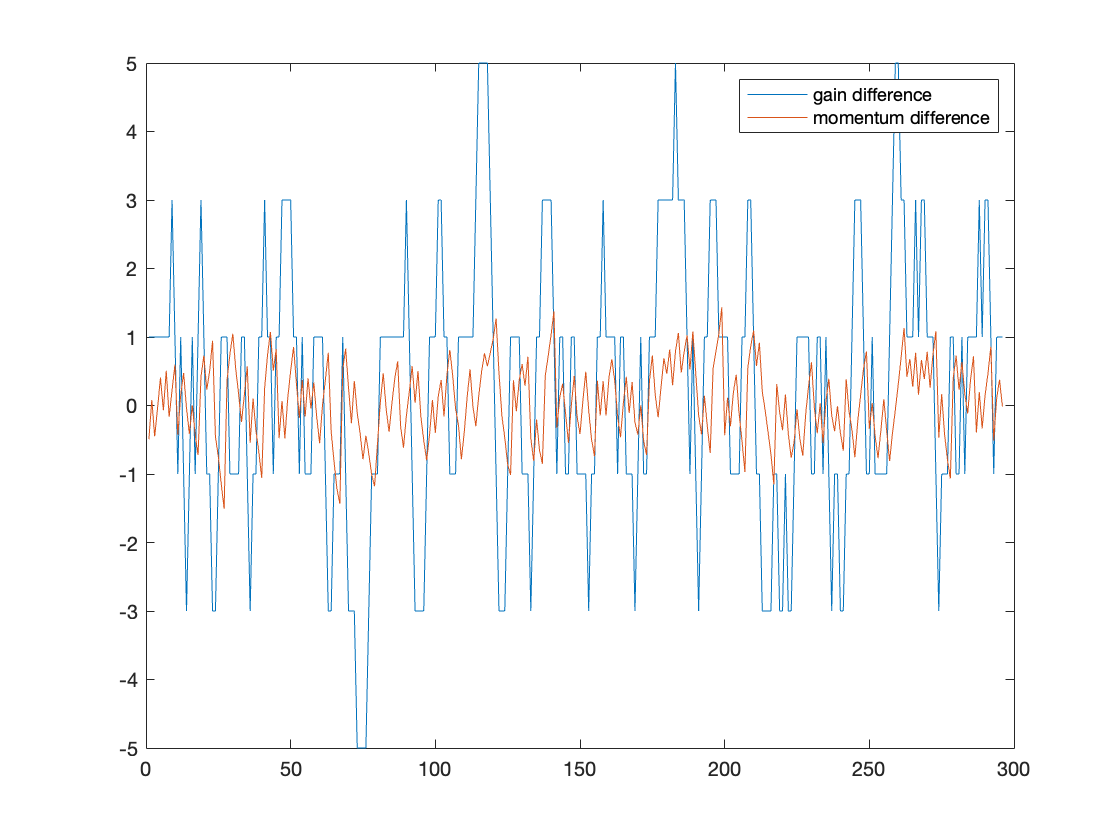
\includegraphics[width=\linewidth]{mainmatter/photos/diff_match1.png}
        \caption{2023-wimbledon-1301}
    \end{subfigure}\hspace{-0.02\textwidth}
    \begin{subfigure}[b]{0.34\textwidth}
        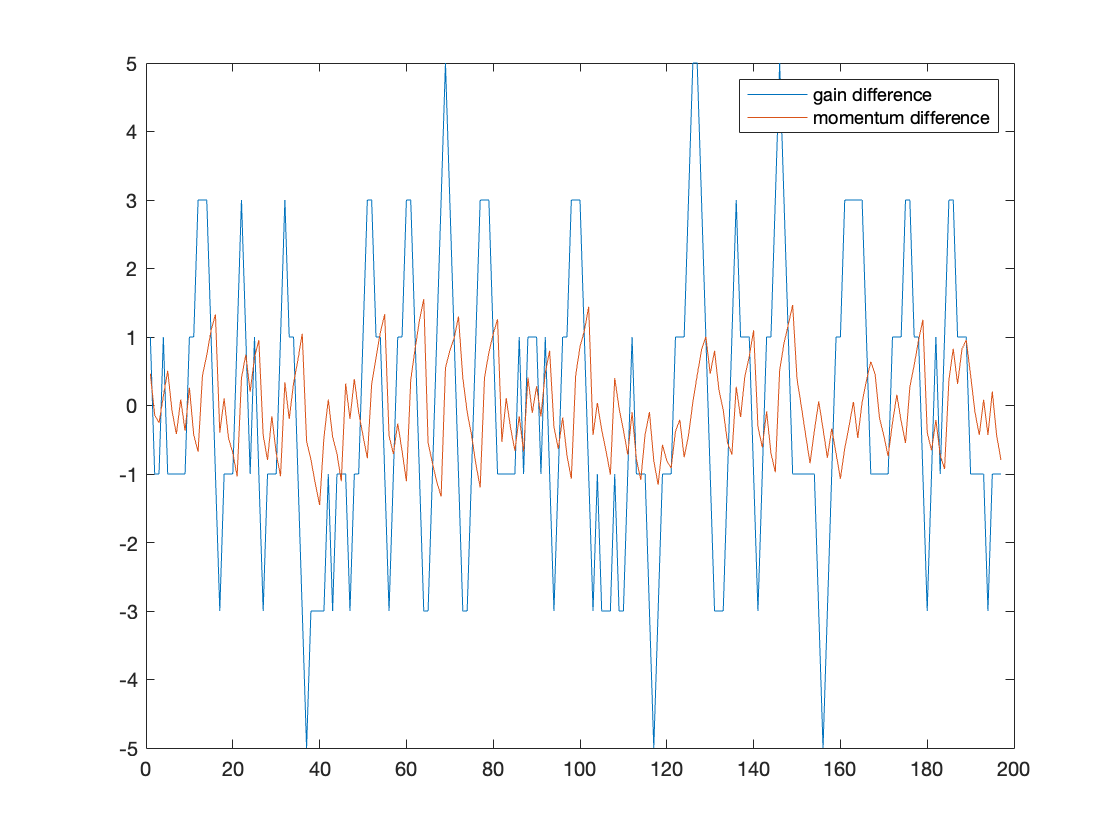
\includegraphics[width=\linewidth]{mainmatter/photos/diff_match2.png}
        \caption{2023-wimbledon-1302}
    \end{subfigure}\hspace{-0.02\textwidth}
    \begin{subfigure}[b]{0.34\textwidth}
        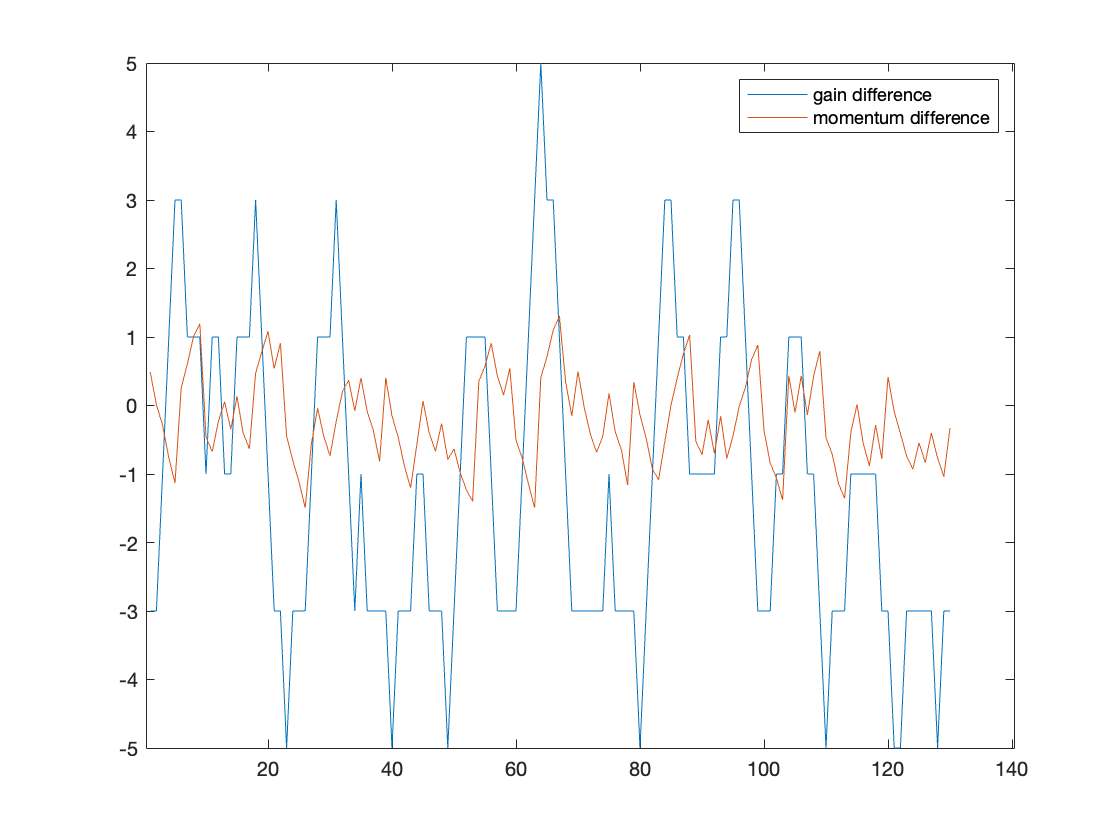
\includegraphics[width=\linewidth]{mainmatter/photos/diff_match3.png}
        \caption{2023-wimbledon-1303}
    \end{subfigure}
    \caption{Gain Difference and Momentum in First Three Games}
    \label{fig:Gain Difference and Momentum}
\end{figure}

And derive the correlation between gain difference from one to five rounds 
and momentum difference of all matches. Here we display the three of them.

\begin{figure}[htbp]
    \centering
    \begin{subfigure}[b]{0.34\textwidth}
        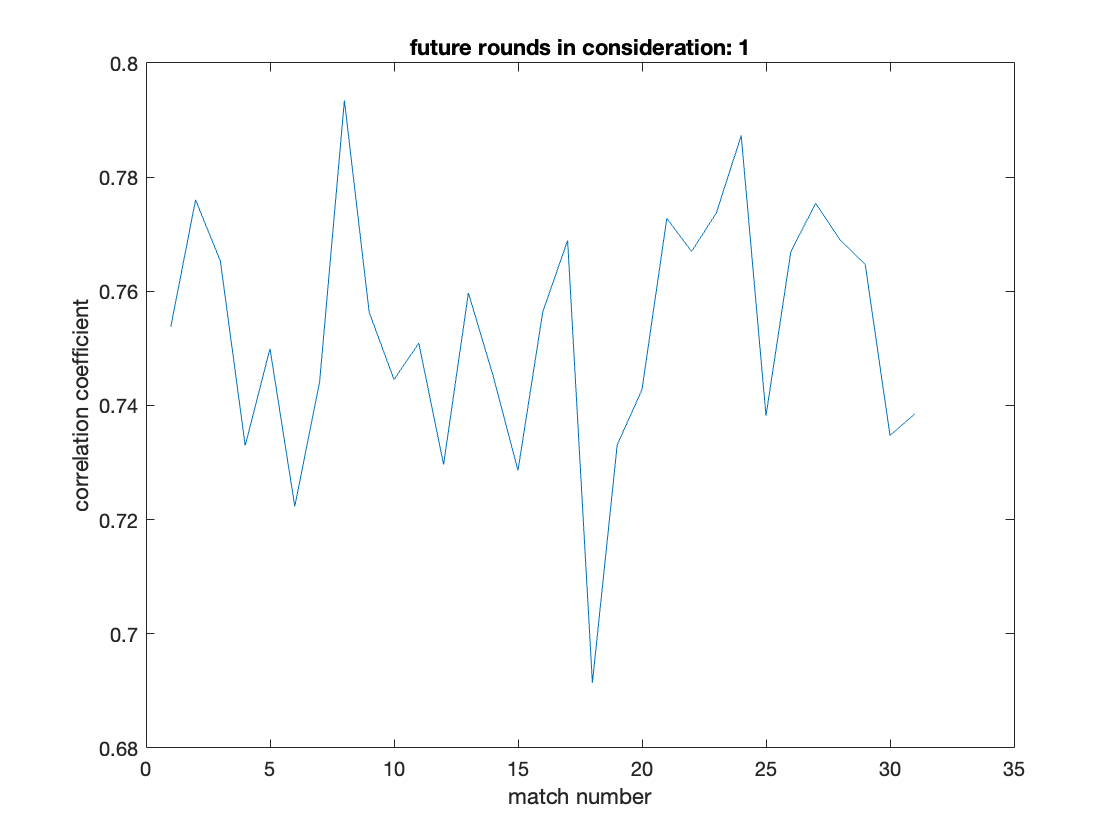
\includegraphics[width=\linewidth]{mainmatter/photos/momen_1points_cor.png}
        \caption{gain difference in 1 round}
    \end{subfigure}\hspace{-0.02\textwidth}
    \begin{subfigure}[b]{0.34\textwidth}
        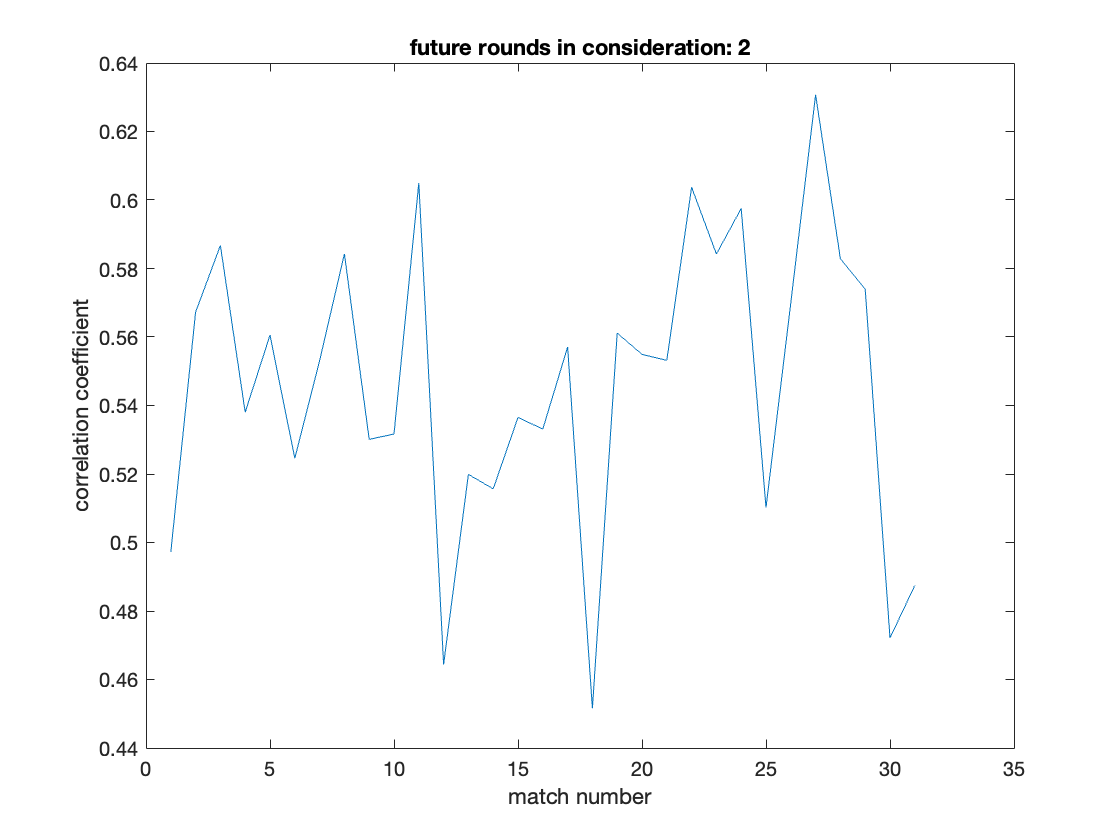
\includegraphics[width=\linewidth]{mainmatter/photos/momen_2points_cor.png}
        \caption{gain difference in 2 rounds}
    \end{subfigure}\hspace{-0.02\textwidth}
    \begin{subfigure}[b]{0.34\textwidth}
        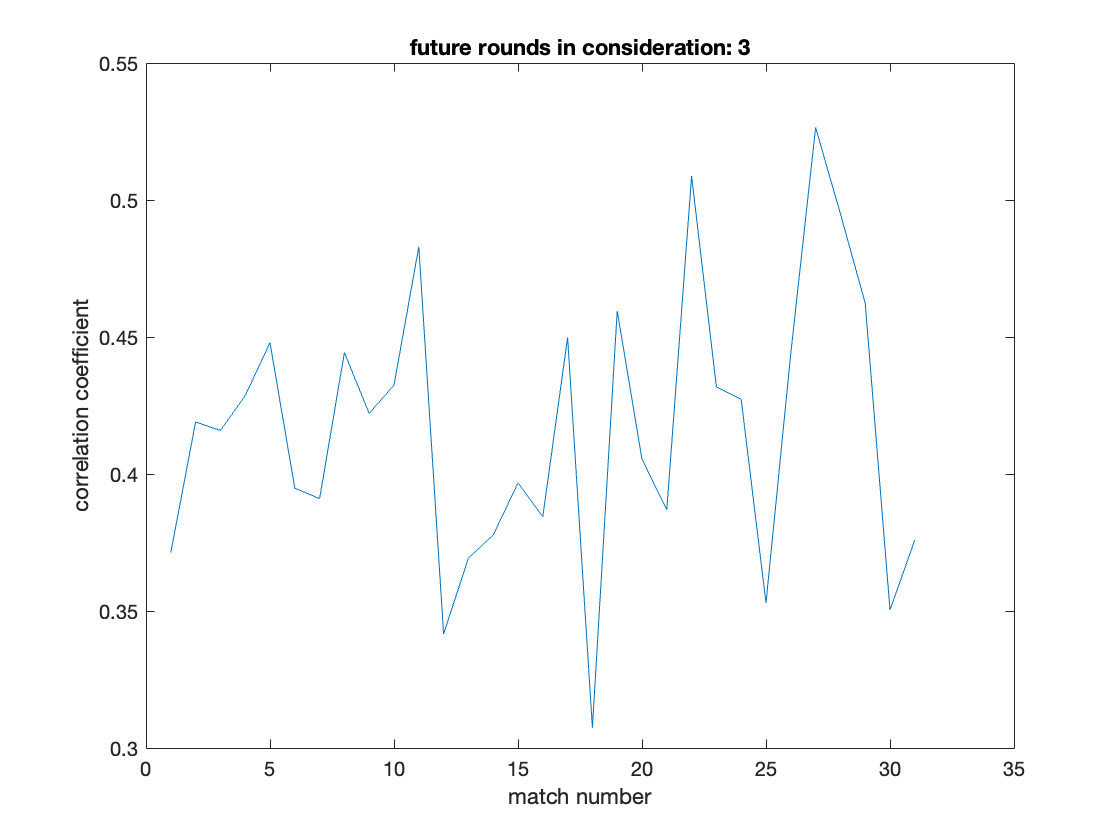
\includegraphics[width=\linewidth]{mainmatter/photos/momen_3points_cor.png}
        \caption{gain difference in 3 rounds}
    \end{subfigure}
    \caption{Correlation Between Gain Difference and Momentum Difference}
    \label{fig:Correlation}
\end{figure}

Here we display the max and min correlation in different rounds.
(hint. the max and min correlation means maximum of all matches.)

\begin{table}[!ht]
    \centering
    \begin{tabular}{|l|l|l|l|l|l|}
    \hline
        rounds & 1 & 2 & 3 & 4 & 5 \\ \hline
        max & 0.7934 & 0.6307 & 0.5264 & 0.4678 & 0.3910 \\ \hline
        min & 0.6914 & 0.4516 & 0.3074 & 0.1824 & 0.0627 \\ \hline
    \end{tabular}
    \caption{max and min Correlation of all matches in different rounds}
    \label{fig:maxmin Correlation}
\end{table}

As we can see from the table, the correlation between momentum and future scores is bigger
than 0.5 considering the next 1 round, it implies that momentum has a substantial impact on the future scores.
And the correlation decreases as the rounds extend, which verifies our intuition, that
the momentum at this moment has less impact on the future rounds as time extends.

Now, we have finished problem 2.